%%
%% This is file `example/ch_concln.tex',
%% generated with the docstrip utility.
%%
%% The original source files were:
%%
%% install/buptgraduatethesis.dtx  (with options: `ch-concln')
%% 
%% This file is a part of the example of BUPTGraduateThesis.
%% 

\chapter{主题建模介绍}
本章将总结一下已有的主题模型方法,以及其发展概况,并探讨其目前仍未解决的问题。
\section{主题模型技术发展概况}
主题模型从一组文档生成主题,并将主题分配给这些文档。基于这些主题,我们可以解决跨域文本分类\cite{Barathi},理解文本聚类\cite{TopicClust},文本推荐和其他相关文本数据应用的问题。虽然对主题模型存在着非凡的研究,但大多数研究集中于基于概率潜层语义分析(PLSA)\cite{PLSI}和潜层狄利克雷分布分析(LDA)\cite{LDA}改进的生成模型。
\subsection{PLSI和LDA的介绍}
主题建模中的最先进的方法是去尝试拟合文集中的文档的生成模型的参数的值。研究生成模型的第一个主要尝试是概率潜层语义分析(PLSA)\cite{PLSI}。目前的黄金标准是潜层狄利克雷分布分析(LDA)\cite{LDA}。第一次,主题模型提供了一种用于聚类文本文档的原则性方法,具有一组明确的假设。这种方法刺激了一系列的研究,旨在推广模型和放松他们的假设。

基于PLSA和LDA算法的生成模型假设每个主题由特定词使用概率分布表征,并且语料库中的每个文档是从主题组合体生成的。作为示例,考虑从两个主题,数学和机器学习领域生成的文档的语料库。图. \ref{fig:TopicModelDoc} 
 \begin{figure}[!h]
\centering
  \includegraphics[width=0.8\textwidth]{./graph/TopicModel.png}\\
  \caption{文档中的文档的生成模型假定是主题的组合体。主题结构是潜在的,意味着人们不能访问用于在语料库中生成文档的“真实”主题集合。然而,可以使用主题模型算法来估计主题集合的分布。为此,在该示例中,计算每个文档中的词频率并将它们建模为不同主题,数学和机器学习的组合体。}\label{fig:TopicModelDoc}
\end{figure}
语料库中的每个文档将从具有特殊概率的主题集中依据这些主题分布抽取单词组成文档。例如,一个文档 $d_{math}$ 主要来自于数学主题的概率是$p(topic = math|d_{math}) = 0.8$ 来自于机器学习的概率是$p(topic = ml|d_{math}) = 0.2$.

具有不同主题组合体的文档将使用不同的词,因为使用给定词的概率分布取决于主题。重要的是,假设一些单词将与单个主题密切相关,否则,将不可能拟合该模型。例如,诸如“loss”或“optimization”的词将主要用于机器学习聚焦的文件中,因为$p(word = loss|topic = machine learning >> p(word = loss|topic = math)$。相比之下,诸如“evolution”或“equation”的词将主要用于数学聚焦的文档中,因为$p(word = evolution|topic = machine learning) << p(word = evolution|topic = math)$。然而,会有其他词,如“research”或“vector”,是通用的,并且两个主题几乎相同。在实践中,人们只能访问每个文档中的字数,而实际的主题结构是不可观察的,即潜在的。因此,挑战是估计主题结构,其由概率集合$p(topic|doc)$和$p(word|topic)$来定义。

为了具体的解释这个问题,我们假设由N个文档组成的语料库使用$N_w$个不同的单词从$K$个主题生成。然后,需要估计$N \cdot K$个概率$p(topic|doc)$和$K \cdot N_w$个概率$p(word|topic)$。PLSA和LDA都旨在估计具有产生数据的最大化似然可能性的这些$K \cdot (N + N_w)$个概率的值\cite{PLSI}\cite{LDA}。因此,PLSA和LDA依赖于非线性地依赖于大量变量的非线性最大化,即非确定性多项式时间难问题。

两个模型之间的主要区别在于,对于PLSA,$N \cdot K$个概率是自由参数,其必须直接从数据中估计,而LDA假设概率集合是从狄利克雷分布中抽取的随机变量[34]。因此,对于LDA,只需要估计$K$个参数(每个主题一个){$\alpha_1; \alpha_2; ...; \alpha_K$}。这些$\alpha$称为超参数。LDA的参数数量通常被进一步减少,假设所有超级主体采用相同的值,通常由$\alpha$表示。假定超级单元的单个值的LDA的“版本”被称为对称LD​​A,而具有K个超级单元的完整模型被称为非对称LDA\cite{ComplexityOfLDA}。
\subsection{PLSI和LDA存在的问题}
\subsubsection{先验的敏感性}
如上一节中所解释到的,LDA和PLSI都旨在依据产生语料库的最高可能性来估计概率分布$p(topic|doc)$和$p(word|topic)$。因此,推理问题被转换为优化问题\cite{ProbabilisticTopicModels}。但是对于同样的文档集存在许多具有几乎相同的可能性的竞争模型。由于似然度的高度退化,标准优化算法将更有可能在不同的优化运行之后推断不同的模型,而不是推断具有最高似然性的模型。因此对于LDA先验尤其重要。在LDA研究的前沿文章\cite{RethinkingLDA}中,深入的讨论了先验对LDA的影响,并做了相当客观的实验证明了其结论。其实验表明非对称的LDA性能优于狄利克雷先验参数用均匀初始化的LDA,然而,值得研究为什么这种非对称的先验提供了卓越的性能。

主题建模的主要假设是主题应该捕获语义相关的词共现。主题也必须是独特的,以传达信息:知道只有少数同时出现的单词应足以解决语义环境。因此,我们不希望特定主题在单词上的分布与任何其他主题类似。因此,非对称先验$\alpha$超过均匀的$\alpha$是一个坏主意:基本量度将反映语料库的词使用统计,并且先验地,所有主题将展现这些统计。一个对称的先验$\alpha$仅仅使得一个先前的语句(由浓度参数$\beta$确定)关于主题是否将在单词上具有更稀疏或更均匀的分布,因此主题可以自由地作为必要的独特和专门化。然而,仍然需要考虑幂律词的使用。这样做的一种自然方式是期望在给定语料库中的每个文档中,某些单词组将比其他单词出现得更频繁。例如,单词“模型”,“数据”和“算法”可能出现在机器学习会议上发表的每篇论文中。这些假设自然地导致我们经验确定为优越的先验的组合:用于跨文档共享共享性的非对称狄利克雷先验,以及用于避免主题之间的冲突的对称狄利克雷。

虽然Wallach等人的研究结果找到了更好的先验方法提高了LDA的性能,即非对称LDA。但是其文中也提到了我们唯一的观测量单词的分布提供的信息并未被LDA这个模型充分的使用。
\subsubsection{主题数目$K$的选择问题}
与此同时,选择主题的数量$K$是有限主题建模中最有问题的建模选择之一。对于迄今为止的$K$的各种值,没有用于选择$K$或评估保持数据的概率的有效方法。并且LDA对于$K$的不良设置是鲁棒的程度尚未被充分理解\cite{RethinkingLDA}。理想情况下,如果LDA有足够的主题来对数据集进行良好建模,则$K$的增加不会对令牌到主题的分配造成影响。即,应该以低频率使用附加主题。例如,如果二十个话题足以准确地建模数据,则通过将话题数目增加到五十个,所推断的话题分配将不会受到显着影响。如果是这种情况,使用大的$K$将不具有对推断的改进。换句话说,我们仍然需要一个健壮的$K$。实际上,$K$可以看作是主题生成的解决方案空间的秩。设置$K$等价于人工选择解空间的秩,这显然是不合理的。

虽然LDA和PLSA之类的图形模型已经催化了无监督学习的大量研究,并取得了许多实际成功,但重要的是要注意,大多数图形模型文献都集中在参数模型上。 特别地,图形和包括图形模型的局部势函数被视为固定对象; 它们在结构上不增长,因为观察到更多的数据。 因此,尽管非参数方法主导了监督学习的文献,但参数方法在无监督学习中占主导地位。 这似乎令人惊讶,因为无监督学习问题的开放性质似乎特别与非参数哲学相称。 但它反映了无监督学习的基本张力,以获得一个良好的学习问题,有必要强加假设,但假设不应该太强烈,或他们将通知发现的结构,而不是数据本身。

而近期主题模型方向的研究中,研究主题数目$K$依然占有相当大的比重,研究者逐渐开始结合数据本身设计先验来试图找出在推断主题模型之前找出合适的主题数$K$或者是找出有效评价主题数$K$的方法。
\section{本章小结}
本文在此章节主要简略的介绍主题模型方向研究的发展过程,之后深入的讨论了主题模型研究需要解决的问题,以及本文对此的一些观点。介绍部分介绍了主题模型的思路源头和要解决的问题并简略介绍了经典的PLSA和LDA方法,在后面的讨论部分介绍了主题模型的先验敏感性和主题数目$k$的选择问题,这些问题是本文后续提出新的主题建模思路的拟解决目标。

\chapter{分层语义映射的自适应主题生成模型HLSM}
本章在总结了之前的传统主题模型方法的优点和存在的问题后,借鉴复杂网络分析算法映射方程(MapEquation)\cite{MAPEQUATION}的思路,提出了一种新的自动主题生成方法,将重点介绍新的主题生成方法的思路并解释其意义。
\subsection{复杂网络中社区发现和主题模型的联系}
所有主题模型算法的核心是找到适合的概率分布$p(topic|doc)$和$p(word|topic)$使得生成文档的似然度最大,即找到以许多局部最大值为特征的似然函数的全局最大值。这种优化问题也是物理系统中无序系统研究的核心问题\cite{complex1,complex2,complex3}。

而本质上$p(word|topic)$是主题模型推断的核心,$p(word|topic)$是每一个主题下单词的分布,如果我们一开始有一个硬的分布约束,即每个词只能属于一个主题。这样的约束下不同的主题(topic)之间不会存在相同的单词(word)。如果我们将所有的单词(word)看做是一个个节点,并将单词(word)之间用我们可以从数据中观测到的信息链接起来,那么推断其归属于某个主题的过程,就是一个复杂网络中社区发现的问题。是一个当然这是一个非常强的约束,我们的主题生成并不会就此结束,后续会讲解之后的优化过程。
\subsection{分层语义映射HLSM模型介绍}
分层潜在语义映射模型(HLSM)是一种用于主题建模的网络方法。 类似于众所周知的主题模型,每个文档被表示为对潜在主题的组合体。区分HLSM模型和现有主题模型的关键特征是HLSM直接将单词进行分块归属到某一个社区中,并将每个社区定义为\emph{初始}主题,然后细化这些初始主题,因此HLSM是以一种全新的方式来推断概率分布$p(word|topic)$与$p(word|topic)$。
HLSM模型按以下步骤推断主题:
   \begin{figure}[!h]
\centering
  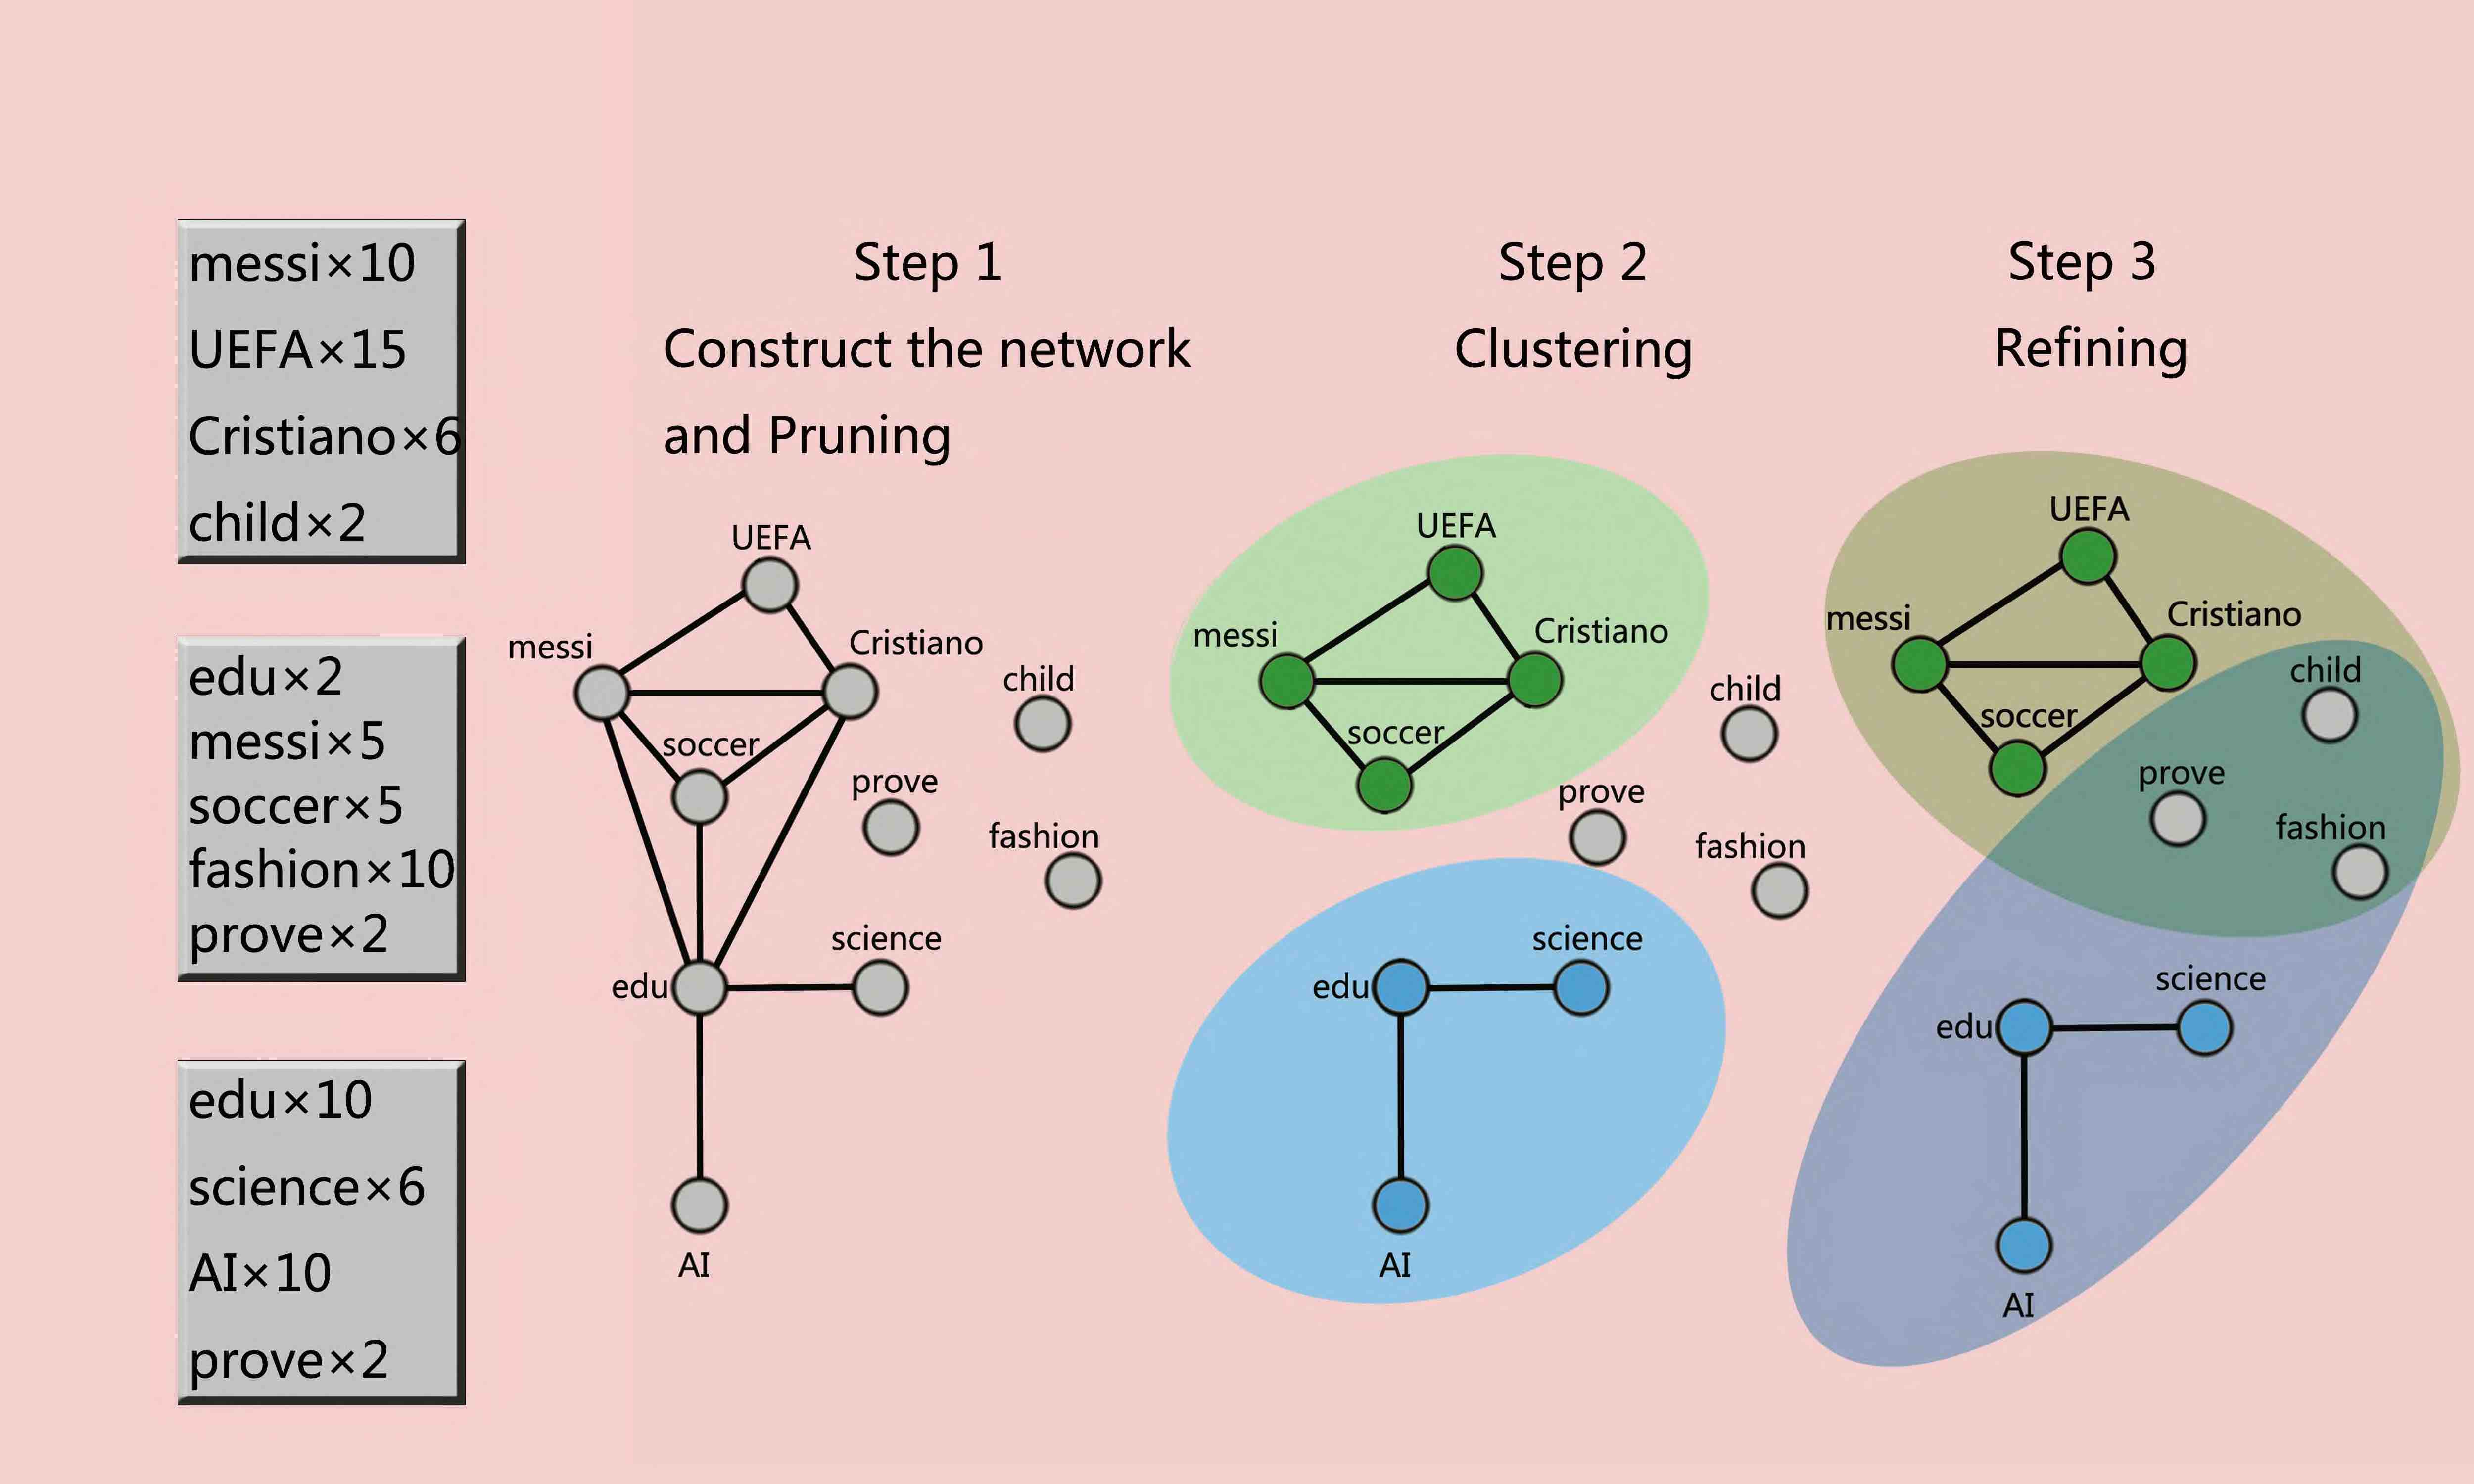
\includegraphics[width=1.0\linewidth]{./graph/hlsmJPG.jpg}\\
  \caption{Illustration of the HLSM algorithm.}\label{fig:hlsm}
\end{figure}
\begin{enumerate}[步骤 1.]
\item \emph{构建单词连接网络}。依据文档集中可观测到的各个文档和单词的共现矩阵构建以单词(word)为节点的带权网络。我们通过单词在各个文档中的分布,计算所有至少在一个文档中共同出现过的两个词(单词对)之间的关联程度值作为其连接的权值。然后,我们将其中单词之间连接权值在一定阈值以上的连接线保留,其余的减枝。
\item \emph{分层地对单词进行社区归属}。通过在潜在主题空间中的关联来连接整个文档集中的单词。自然地,我们假设语料库中的主题将引起网络中的单词的社区。因此,我们使用分层信息映射方程(Hierarchical Map Equation)\cite{HME}来检测社区。在大多数语料库中,主题以多级抽象的形式出现。抽象主题下又包括几个具体主题。因此,我们检测到对应于抽象主题的一些大规模社区,然后我们检测来自大规模社区的小社区,这对应于更为具体的主题。我们采用社区作为对用于生成文档的每个主题的主题数量和单词组成的\emph{初始}猜测。值得注意的是,我们不人工设置总共的层级数量每个层级社区的数量。分层信息映射方程可以自动揭示单词网络中的多级组织。
\item \emph{优化初始的概率估计}。在最后一级的单词聚类之后,我们可能会发现一些社区和别的社区都没有连接,并且在步骤2中,也可能得到可以得到不在网络中的单个单词。并且,合理的主题模型不应该所有的单词都只能属于一个主题,单词因此,在步骤2中检测到的先前主题是非常粗糙的,我们使用类似PLSA的似然优化来改进这些粗糙的\emph{初始}主题。
\end{enumerate}

\subsubsection{构建单词连接网络}
词之间的关联权值必须与主题密切相关,以确保基于该网络对词进行社区归属的有效性。但主题是潜在的,所有的观察都是收集到的文档中的单词的分布。现在假设我们用之前的人类知识人工地分配主题,人们可以观察到共享相同的主题文档会有更大的概率共享一些单词。自然地,我们可以认为在许多文档中共同出现的词语共享相同的主题,换而言之,这些词语在潜在主题空间中更为相似。

为了计算潜在主题空间中的单词之间的关联,与潜在语义分析(LSI)的核心思想一样,我们基于共生矩阵$ M $的\emph{奇异值分解}(SVD)将单词映射到降维的向量空间,其中每一行$ i $对应于一个单词,每一列$ j $对应于一篇文档,并且每个矩阵条的元素$ M_{ij} $对应于文档$ j $中单词$ i $的出现次数。
  
  
整个过程开始于标准的SVD:
    \begin{equation}
  M = U \Sigma V^t,
   \end{equation}      
对角矩阵$ \Sigma $包含M的奇异值。$ M $的近似值是通过将$ \Sigma $中的所有最大$ K $个奇异值设置为零来计算的(= $ \widetilde{\Sigma} $ ),其意义是在$ L_2 $ 范数空间上秩为$K$的表达。

现在获得了M的一个近似矩阵
    \begin{equation}
    \widetilde{M} = U \widetilde{\Sigma} V^t  \approx  U \Sigma V^t = M,
   \end{equation} 
   
原始高维矩阵$ M $是稀疏的,但是相应的低维潜在向量通常不是稀疏的。这意味着我们可以更好的通过这些低维空间计算潜在主题空间中的单词对之间的有意义的关联值,而不是简单的将单词对之间的共现(在同一个文档中出现)次数当做被构建的单词网络的权值。 在HLSM中,我们计算$ U\widetilde{\Sigma}$的行之间的余弦距离作为潜在主题空间中每对词的关联值,并且将词$ i $和$ j $与该关联连接$ S(i,j)$:
      
   \begin{equation}	
    W = U\widetilde{\Sigma},\\
   S(i,j) = \frac{\langle W_i \cdot W_j \rangle }{ \| W_i \| \cdot \| W_j \|}.
   \end{equation}
   
计算完所有共现单词对的关联值后,我们对整个构建的单词网络进行剪枝。一些共现词对之间的关联值非常低,我们可以假设这些连接是噪声。因此设置$ q $的阈值以使关联权值低于$ q $的边被除去。

\subsubsection{分层地对单词进行社区归属}
在大多数语料库中,主题的结构并不是简单的单层结构,总是可以有多个层次。一些具体的主题在同一个抽象主题下。例如,集中在“足球”上的语料库中的词语可能来自“名星”,“竞赛”,“足球史”等主题。

我们基于潜在主题空间中的词之间的关联来构造词的网络。如果主题的原始结构是多级的,则网络也应该具有多级结构。要在上一节中建立的单词网络中发现多个级别的社区,我们选择\emph{Hierarchical Map Equation} \cite{HME}。值得注意的是,我们没有人工的为每个级别设置级别数量和社区数量。相反,层次映射方程\cite{HME}可以通过这个模拟信息流在网络中的随机游走,并通过类似贪心的算法,自动揭示单词网络中的多级结构。
 
映射方程(Map Equation)提出了寻找网络中的社区结构和最小化表达随机游走者在网络上的移动的编码长度之间的对偶性。对于给定的网络分区,映射方cite程定义了在理论上可以描述该随机游走的轨迹的最短编码长度$ L(M)$。映射方程的核心思想是,如果随机游走者倾向于长时间停留在网络的一些分区中,则可以通过在这些分区内部的节点上公用一个表达分区的编码,从而减少表达整个网络中每一步游走所需的平均编码长度。其本质,是通过规定了分区的划分,从而减少了整个网络的不确定性,也就是表达整个网络的熵。因此,当用于网络中的实际流随机游走时,在所有分区可能的网络分区上估计最小表达编码长度$L(m)$可以依据网络中随机游走的动力结果揭示网络本身的结构。
 
  
在主题建模的问题中,对应于$n$个节点的分层网络$ M $,每个节点对应一个单词(word),被划分为$ m $ 个分区。在每一个分区中有一个拥有$ m^i $个子分区的子映射$ M ^ i $。相应地,在每个子分区$ij $中有一拥有$ m ^ {ij} $ 个子分区的个子映射$ M ^ {ij} $,以此类推。

对应的层级映射方程$L(M)$是
 \begin{equation}
  L(M) = q_{switch}H(Q) + \sum_{i=1}^mL(M^i)
  \end{equation}
 中间级别的子映射$M^i$的映射方程
   \begin{equation}
  L(M^i) = {q^i}_{switch}H(Q^i) + \sum_{j=1}^{m^i} L(M^{ij})
  \end{equation}
  最底层即最细粒度的映射方程
  \begin{equation}
  L(M^{ij...k}) = {p^{ij...k}}_{in} H(P^{ij...k})
  \end{equation}

每个码本的权重取决于码本的使用比率,并且$ L(M)$是每个码本的码字的平均长度的和。 $ H(Q)$是根据其使用率的索引码本中的码字的平均长度,而熵项取决于码本被使用的比率。在任何给定步骤上,随机游走者以$ q_ {switch} $的概率切换\emph {第一}级分区,而$ q_ {switch} $是使用索引码本的比率。
  
在每个子分区级别,$ H(Q ^ i)$是根据子索引码本中的使用比率的码字的平均长度,并且$ q_ {switch} ^ i $是用于进入$ m_i $子分区或退出到更高级别的码字使用比率。在最后一级, $H(P^{ij...k})$ 是对应于子分区码本中的使用比率的平均编码长度,$ p({ij ... k} _ {in} $是子分区$ij...k$中随机游走的代理访问节点或者跳出到其他子分区的比率。找最好地表示结构的分层结构的问题被转换为找到具有最小映射方程的网络的分层分区。图\ref{fig:mapequation}说明了一个映射方程的例子。
\begin{figure}[!h]
\centering
  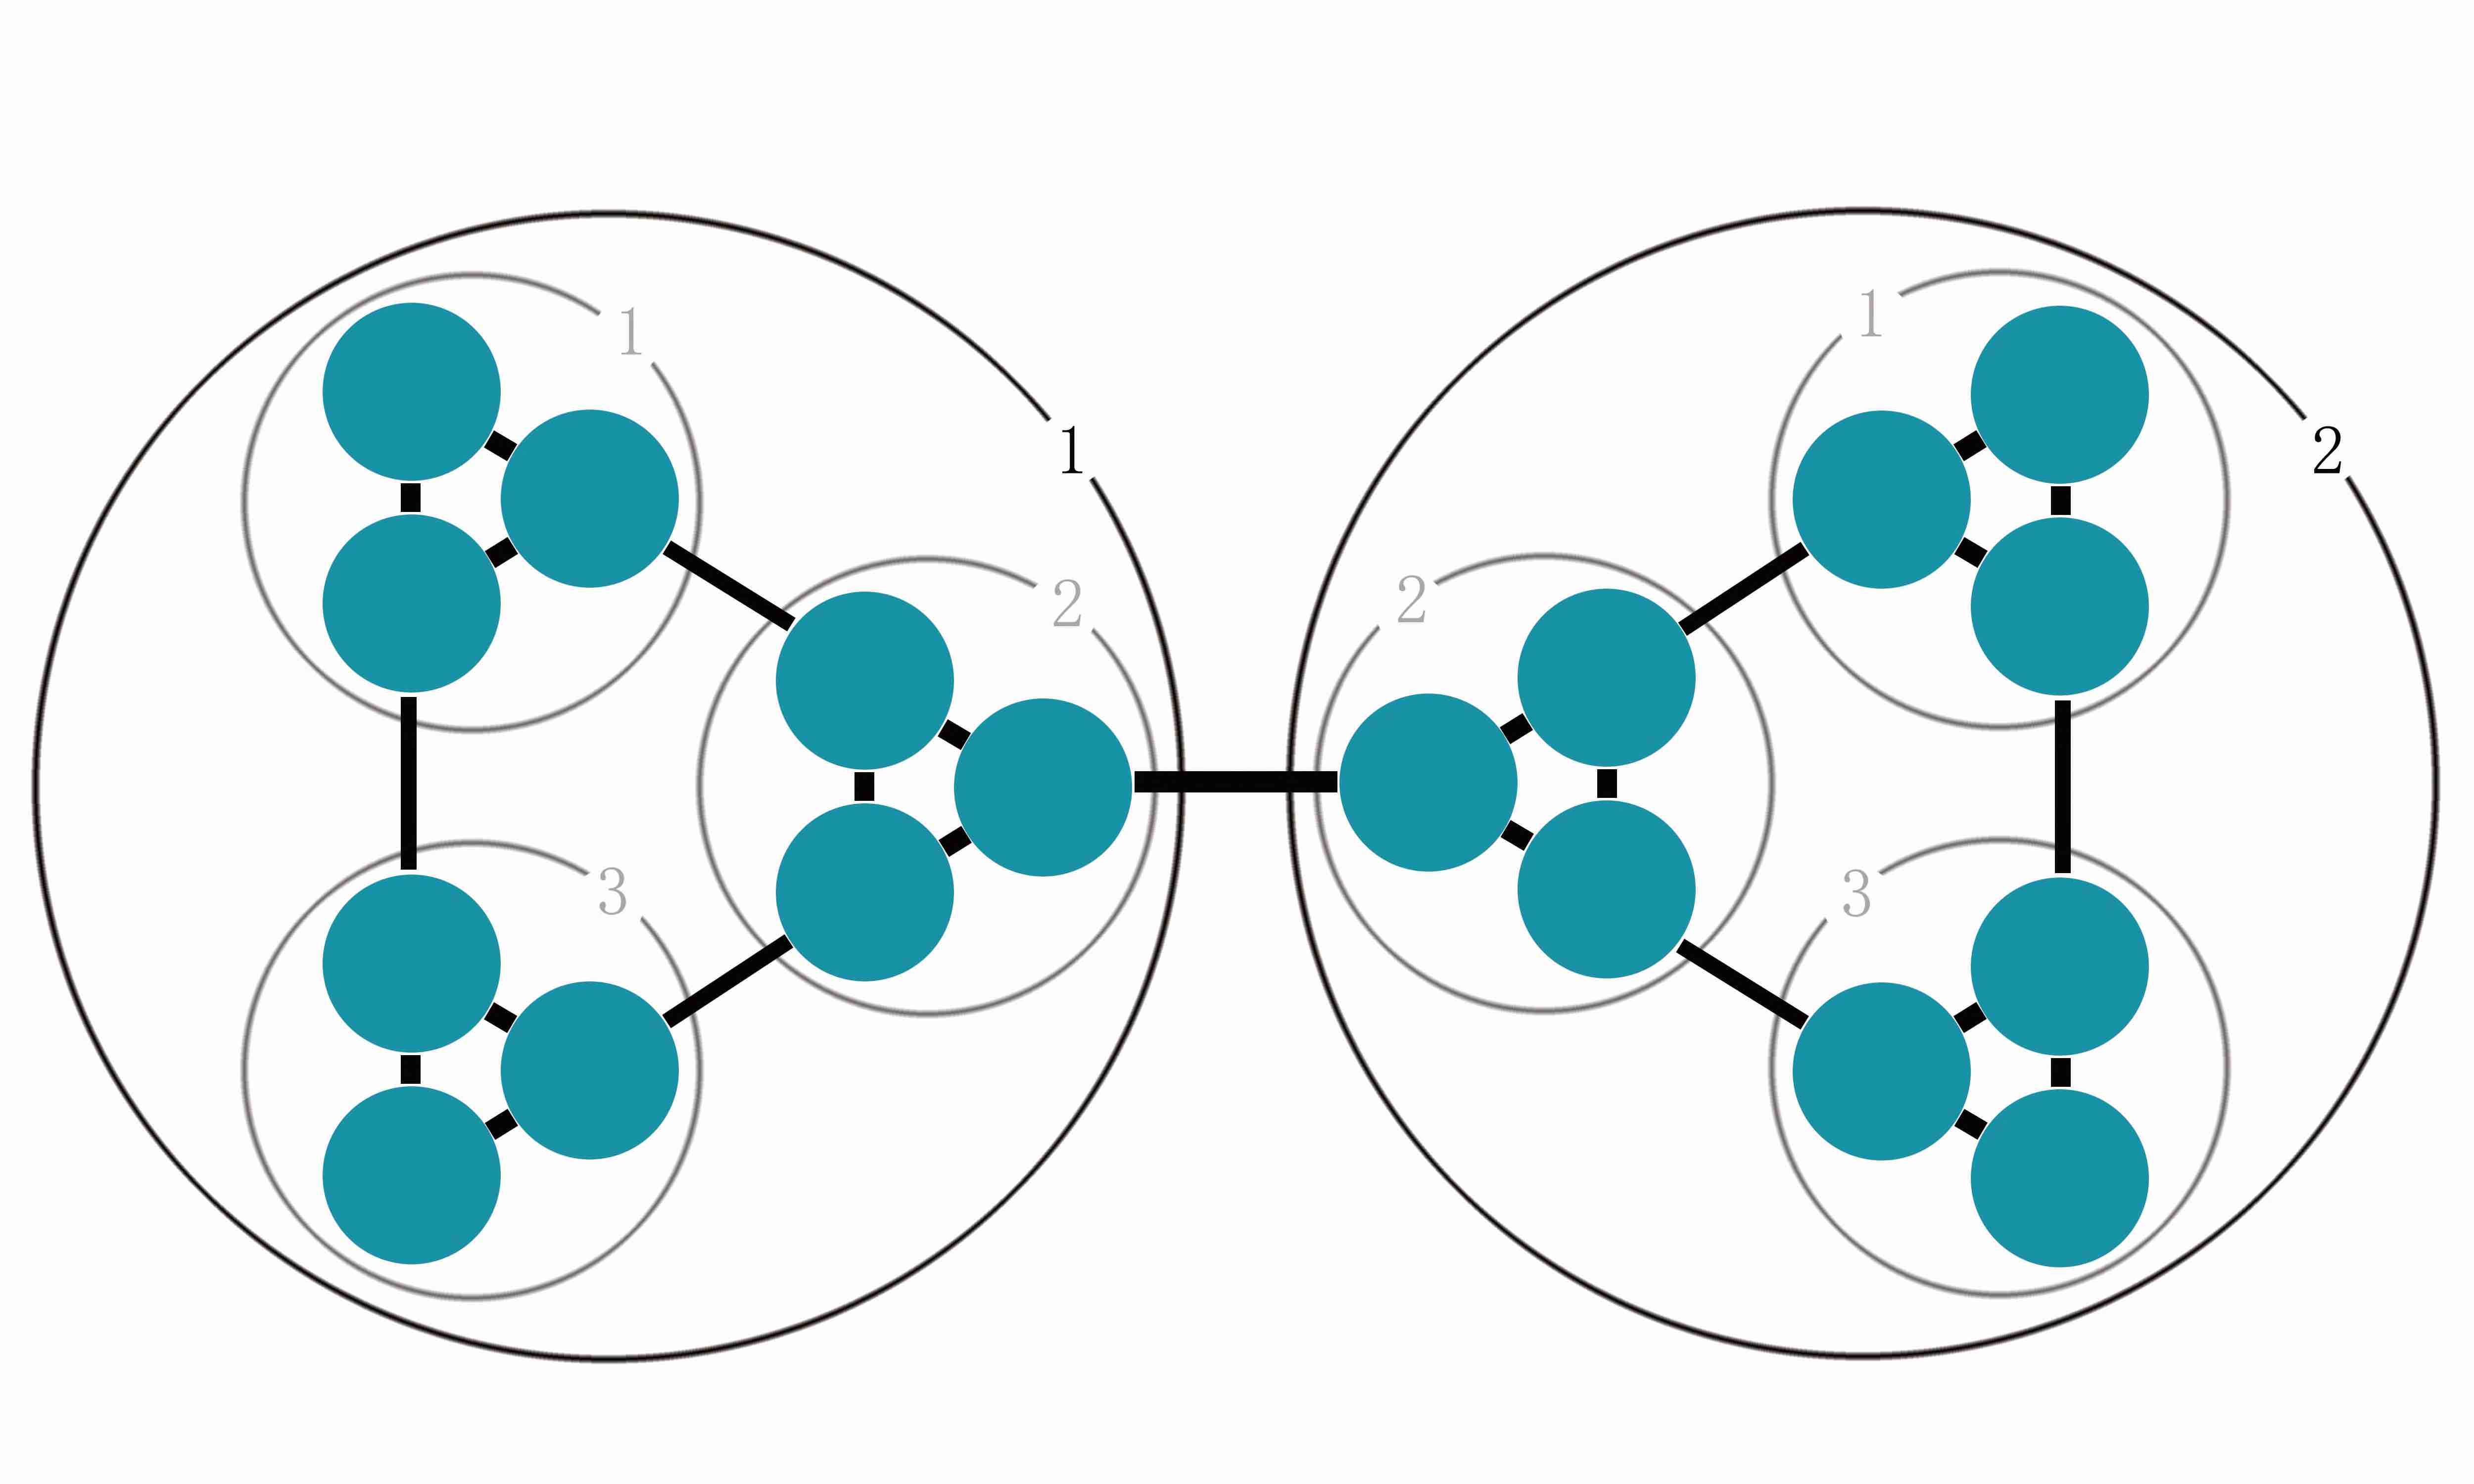
\includegraphics[width=1.0\textwidth]{./graph/mapequationJPG.jpg}\\
  \caption{通过最小化映射方程来找到对应于网络中最优分区结构的例子。}
\label{fig:mapequation}
\end{figure}

在这个例子中,我们可以假定网络中连接的所有权重是相等的,因此所有比率都可以通过计算连接边的数量和归一化来得到。未分区网络的映射方程(平均表达编码长度)为$ - log_2(1/18)= 4.17 bit$。在网络被分区后,第一级分区的码字以总比率$ q_ {switch} = \frac {2} {50} $被使用(考虑移动方向时,网络中有25条线路和50个可能的移动,而只有2个移动可以在第一级分区之间切换),同时第一级的两个分区的使用比率就是$ Q = \frac {1} {2},\frac {1} {2} $。 同时分区1内的子分区使用比率分布$ Q ^ 1 = \frac {2} {8},\frac {2} {8},\frac {3} {8},\frac {1} {8} $, $ \frac {1} {8} $ ,注意一点,随机游走的代理有可能以$ q_ {switch} ^ 1 = \frac {8} {50} $的概率从分区1跳转入分区2。 因此$ L(M)$是:\\
\begin{equation}
%\begin{small}
L(M) = q_{switch}H(Q) + \left\{
\begin{aligned}
q_{switch}^1H(Q^1) & + & \left\{
\begin{aligned}
p_{in}^{11}H(P^{11}) \\
p_{in}^{12}H(P^{12}) \\
p_{in}^{13}H(P^{13}) \\
\end{aligned}
\right.\\
q_{switch}^2H(Q^2) & + & \left\{
\begin{aligned}
p_{in}^{21}H(P^{21}) \\
p_{in}^{22}H(P^{22}) \\
p_{in}^{23}H(P^{23}) \\
\end{aligned}
\right.
\end{aligned}
\right.
%\end{small}\\
\end{equation}\\
\subsubsection{优化初始的概率估计}
一旦网络建立,我们使用\emph{分层映射方程(Hierarchical Map Equation)}来检测高度关联词的簇(与由\emph{分层映射方程(Hierarchical Map Equation)}检测到的分区相同)。在\emph{最后}一层分区探索完全之后,我们得到一个对单词非常硬的分区,意味着单词只能属于一个单一的分区。而这里的每一个分区对应我们的主题建模问题,是一个初始的主题。实际上,一个词在不同的上下文中可能具有多种意义和多种类型的使用。因此,如果我们简单地将每个分区定义为一个主题,这些粗略的主题不能提供关于语料库对应于潜在主题空间的合理的概率解释。因此,我们提出了一种进一步改进这些粗糙\emph{初始}主题的方法。

我们现在讨论如何在给定了每个词属于的一个主题(分区)后去计算$ p(topic | doc)$和$ p(word | topic)$。在之前的单词分割中,我们将每个分区定义为一个主题。事实上,在\emph{分层映射方程(Hierarchical Map Equation)}处理之后,网络中的每个单词(word)都只能位于一个分区中。因此,$ p(t | w)= \delta_{t,w} $。 $ \delta_{t,w} = 1 $,如果单词$ w $位于对应于主题$ t $的分区中。对于其他主题$ \bar{t} $,$ \delta_{\bar{t},w} = 0 $。注意到在这一步中,词$ w $只能属于一个主题t,所以$ p(w,t)= p(w)$,同时 $p(t|d) = \frac{\sum_wp(t|w)}{L_d}$因此:
   \begin{equation}
   p(w|t) = \frac{p(w)} {\sum_w p(w)\times \delta_{t,w}}  \mbox{    and    }  p(t|d) = \frac{1}{L_d} \sum_{w} w_w^d \delta_{t,w} .
  \end{equation}
  
其中$ L_d $是文档$ d $中的单词数,$ w_w^d $是单词$ w $出现在文档$ d $中的次数。$n(w,t) = L_C \times p(w,t)$是在生成整个语料库时主题$ t $被选中后,从主题$t$的所有单词中选中单词$w$的次数。$ L_C $是语料库中的单词的数量。
所以目前为止,我们的主题模型的类似PLSA的似然函数为:
 \begin{equation}
 \begin{split}
 L = log (\prod_{w,d}p(w,d)) = log (\prod_{w,d} \sum_{t}p(w|t)p(t|d))  \\= \sum_d \sum_w w_w^d \times log(\sum_{t}p(w|t)p(t|d)) \ .
 \end{split}
 \end{equation}
  
现在文档中的每个词都属于且仅仅属于一个主题,那么整个文档所对应的总的主题数是非常多的,且对应于其中少数词属于的主题,这篇文档可能在这里并不是想表达这个主题的语义。因此我们可以通过简单地使文档中的词更具体的去归属于较少的主题来提高整体生成当前文档的似然度。为此,我们的优化算法简单地为每个文档找到分配有一些不常出现的主题的单词,并将该文档中最重要的主题重新分配给这些单词。  
   \begin{enumerate}[步骤 1.]
  \item 对于每一篇文档$d$, 我们依据最小化$p-value$(后面会介绍)来找到它最\emph{重要}的主题$t_s$。在主题模型中,每个单词$w$都是独立的从每个主题$t$中采样出来的,反过来主题被选中的概率$p(t) = \sum_{w}p(w)p(t|w)$。同时我们把$x$定义为文档$d$中从主题$t$中采样出的单词的个数(主题为$t$的单词的个数),那么依据前文公式(modify)$x = L_d \times p(t|d)$,此时我们可以通过伯努利分布来计算主题$t$的$p-value$,$p-value = B(x; Ld, p(t))$。显然$p-value$对主题$t$在文档$d$中的重要性的表达能力要强于$x$,因为$x$仅仅和$p(t|d)$相关,而$p-value$考虑了整个语料库的信息$p(t)$。
  \item 在构建单词网络的那一步中,对于每一篇文档$d$,都有可能含有一些单词独立在这个网络之外,也就是和所有词都没有共现或者是权值太低连接线被剪枝掉。对于这些单词,我们很简单的将这篇文档中最\emph{重要}的主题当做这些单词的主题,由此我们可以计算一个底线的类似PLSA的似然度$L$(modify).
  \item 对于每一篇文档$d$,我们通过设定了一个参数阈值$\eta$来将那些不常出现的主题$p(t_{in}|d) < \eta$定义为$t_{in}$。同时将前文提到的最\emph{重要}的主题赋予给这些从$t_{in}$选出来的单词。需要注意的是,所有$p(t_{in}|d)$都会被置为0,与此同时$p(t_s|d)$ 会获得所有$p(t_{in}|d)$的和的增长。相应的,$n(w,t_{in})$会减少相对于那些在文档中属于$t_{in}$的单词的数量$w_w^d$,而$n(w,t_s)$获得相应的提高。
  \item 在前面的步骤依次在所有的文档都执行完之后,我们开始计算:
  \begin{equation}
 \begin{split}
 p(w|t) = \frac{n(w,t)}{\sum_w n(w,t)}
  \end{split}
 \end{equation} 同时整个模型的似然度,$L_{\eta}$,在这里和我们定义的参数$\eta$相关。如果最终的目的是要获得最好的模型并且在可以进行交叉验证的场景下,我们简单的通过将$\eta$从0\%到50\%以每步1\%的方式迭代验证,从中一局最大的似然度$L_{\eta}$来选择最终模型,这里是一个很简单的参数寻优过程,只用了简单的交叉验证来寻找并未探索更看起来简便的方法,不过由于后面的迭代计算量并不大,所以对模型的计算开销不大。
  \end{enumerate}

HLSM从训练数据中去预估两个概率分布$p(w|t)$以及$p(t) = \sum_{w}p(w)p(t|w)$,对于一个新的文档,HLSM的推断过程非常简单,固定$p(w|t)$,$p(t|d)$可以通过如下公式计算:
   \begin{equation}
 \begin{split}
 p(t|d) = \frac{\sum_wp(t|w)}{L_d}
 \end{split}
 \end{equation}
 
由于在训练过程(更严格的说法是在训练数据集上推断完概率分布)之后,HLSM固定了$p(w|t)$和$p(t)$,因此HLSM存在较大的过拟合风险,这个在训练集数据比较小的时候会是HLSM的一个缺点。
 
\subsection{评估HLSM性能的实验}
HLSM是一个面向语料库处理的主题模型。它可以应用于许多方向的应用,如文本分类,聚类,过滤,信息检索等相关领域。我们在这里按照Blei的想法\cite{LDA},在本节中,我们考察HLSM和其他传统主题模型在两个重要的应用场景上的应用:文档建模和文档分类。
\subsection{文档建模}
文档建模的根本目的是将训练的模型从训练数据集推广到新的未见过的数据集。语料库中的文档是未标记的,我们的目标是对文档的主题概率分布进行估计,因此我们希望在训练集上表现良好的模型在测试集依然能获得较高的似然度,这样才能证明模型的可推广性。具体来说,我们计算了一个测试集上的\emph{混淆度}来评估模型的性能。产生较低混淆度的模型被认为实现更好的泛化性能,因为这样的建模方法获得的模型在处理该模型从未见过的那部分数据集时不会显得困惑。正式地,对于$ M $个文档的测试集,混淆度被定义为:
  \begin{equation}
  perplexity(D_{test}) = exp \left \{ \frac{-\sum_{i=1}^Mlogp(d_i)}{\sum_{i=1}^ML_i}\right \}
  \end{equation}
   \begin{figure}[h]
\centering
  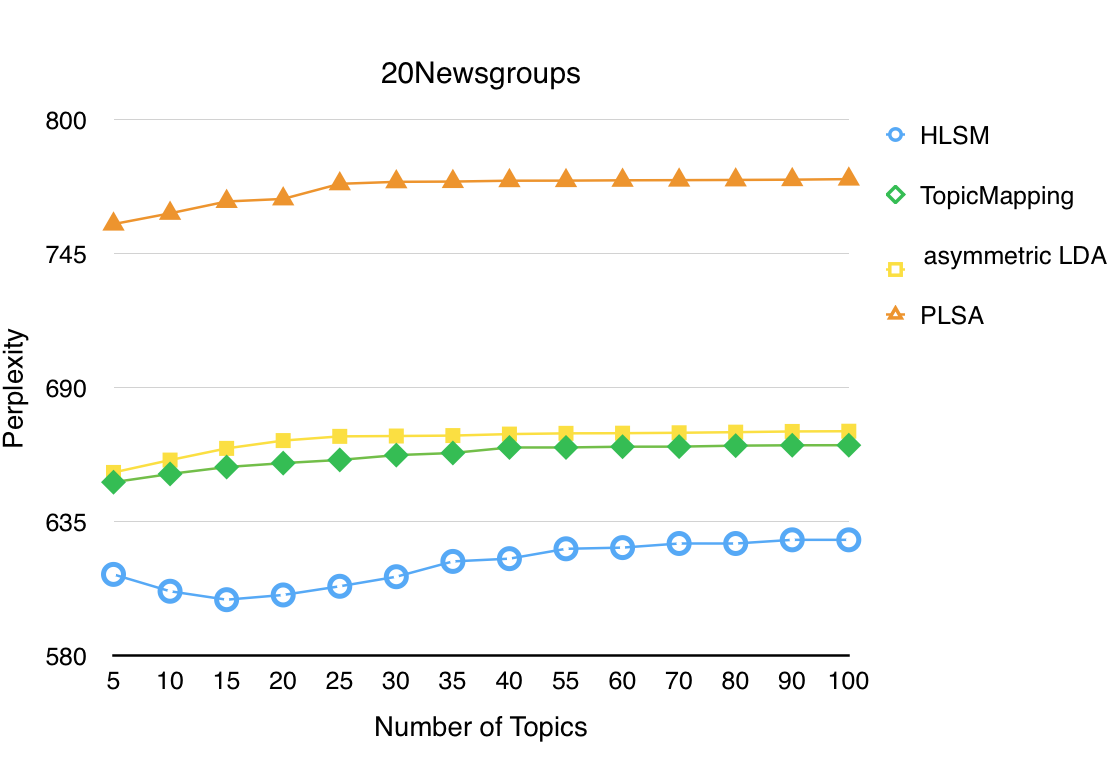
\includegraphics[width=1.0\textwidth]{./graph/perplexitycolor.png}\\
  \caption{Perplexity comparisons on the 20Newsgroups dataset.}\label{fig:perplexity}
\end{figure} 

我们在20Newsgroups数据集的一个子集上进行了这个实验,该数据集已被广泛用于评估跨域文本分类算法的性能。它包含近20,000个新闻组文档,这些文档已被均匀分为20个不同的新闻组。我们选择了3878个文档(我们过滤了一些小文档),来自四个领域:comp.graphics,com.sys.mac.hardware,sci.crypt和sci.med作为我们在评估中使用的数据集。我们随机抽取了20%的语料库用于测试,并在剩余的80%文档中做训练。在数据预处理方面,我们从标准的原始文档中删除了163个停用词,并从每个语料库中删除了出现次数小于3的单词。我们比较了HLSM与PLSA,asymmetric LDA(非对称LDA)和TopicMapping等模型的效果。对于所有主题,asymmetric LDA的初始$\alpha$设置为0.01。
 
图\ref{fig:perplexity}显示了主题数量从5变化到100不同模型的混淆度结果。这里由于HLSM是一个自动寻找到主题数的模型,我们没有去过多调节上一节中提到的唯一的超参$\eta$,而是在计算混淆度的时候如上一节中的迭代优化过程一样循环的将那些在文档中占比小的主题所属词归属到最重要的几个主题内,从而计算5到100个主题数的混淆度。可以看出,HLSM模型在混淆度方面实现了轻微的改善,而TopicMapping接近于不对称LDA。实验表明,HLSM依靠对单词网络构建后的层次分区发现得到的先验猜测在主题生成的性能上有较明显的提高。
 
表\ref{table:topics}提供了HLSM在数据集\emph{Comp \& Sci}上提取的$p(t|d)$最大的12个主题的示例,一些具有较低概率的主题未被展示出来。我们用学习的主题词概率$p(w|t)$对词进行排序。通过检查主题词,我们可以观察到同一主题中的词总是语义相关的。例如,主题1是关于Mac硬件,而数据集\emph{Comp \& Sci}中的一个领域正好是comp.sys.mac.hardware。值得注意的是,一些主题在抽象层面看起来相似,但它们之间在更具体的意义上仍然有一些区别。例如,主题2和主题4中的单词在语义上相关,但主题2与医疗更相关,而主题4可能描述了一些关于疾病的报告。结果表明,我们的方法可以有效地识别来自不同领域的领域特定功能之间的相关性。此外,我们的方法可以提取抽象领域范围内的更为具体或者说更细粒度的的主题。我们还在20Newsgroups数据集进行了下一个实验。

\begin{table*}[ht]
\centering
\caption{Comp and Sci数据集上HLSM生成的Top12个主题的单词分布}
{\scriptsize
 \setlength{\abovecaptionskip}{3pt}
\setlength{\belowcaptionskip}{11pt}
\newcommand{\tabincell}[5]{\begin{tabular}{@{}#1@{}}#2\end{tabular}}
%\centering
%\caption{Examples of Top 12 Topics Extracted by HLSM on Data Set Comp and Sci}
\label{table:topics}
\begin{tabular}{|c|c|c|c|c|c|}
\hline
topic: 1  & topic: 2 & topic: 3 &  topic: 4 &  topic: 5 & topic: 6 \\
$p(t)$ : 0.080127 & $p(t)$ : 0.06720 & $p(t)$ : 0.066154 & $p(t)$ : 0.061912 & $p(t)$ : 0.060678 & $p(t)$ : 0.060007\\
\hline
mac & doctor & clipper & medic & food & imag\\
doe & patient & phone & health & msg & jpeg\\
system & vitamin & chip & 1993 & diet & file\\
speed & medic & encrypt & diseas & eat & format\\
price & candida & govern & hiv & weight & gif\\
hardware & treatment & onli & report & effect & program\\
\hline
topic: 7  & topic: 8 & topic: 9 &  topic: 10 &  topic: 11 & topic: 12 \\
$p(t)$ : 0.056193 & $p(t)$ : 0.055702 & $p(t)$ : 0.050720 & $p(t)$ : 0.046258 & $p(t)$ : 0.045494 & $p(t)$ : 0.044068\\
\hline
imag & drive        & key        & anonym & nsa     & 3d\\
data & disk          & encrypt & email & writes       & graphic\\
system & system & messag & internet & govern & file\\
packag & work     & secur    & post & articl         & object\\
sourc & scsi         & pgp       & comput & david     & ray\\
code & machin   & attack    & inform & trust       & model\\
\hline
\end{tabular}}
\end{table*}

\subsection{文档分类实验}
 \begin{table*}
 \centering
\caption{从20Newsgroups抽取出的数据集}
{\small
\setlength{\extrarowheight}{0pt}
\baselineskip=5pt
\newcommand{\tabincell}[2]{\begin{tabular}{@{}#1@{}}#2\end{tabular}}
%\centering
%\caption{Data Sets Generated from 20Newsgroups }
\label{table:dataset}
\begin{tabular}{|c|c|}
\hline
Data set & Domain\\
\hline
 Comp and Sci & \tabincell{c}{comp.graphics \\comp.sys.mac.hardware \\sci.crypt \\sci.med}\\
\hline
Comp and Talk & \tabincell{c}{comp.os.ms-windows.misc\\comp.sys.ibm.pc.hardware\\talk.politics.mideast\\talk.politics.misc}\\
\hline
Comp and Rec & \tabincell{c}{comp.graphics\\comp.sys.ibm.pc.hardware\\rec.motorcycles\\rec.sport.baseball}\\
\hline
Sci and Rec & \tabincell{c}{sci.crypt\\sci.med \\rec.autos\\rec.sport.baseball}\\
\hline
Talk and Rec & \tabincell{c}{talk.politics.mideast\\talk.politics.misc\\rec.autos\\rec.sport.baseball}\\
\hline
Talk and Sci & \tabincell{c}{talk.politics.misc\\talk.religion.misc\\sci.crypt\\sci.med}\\
\hline
\end{tabular}}
\end{table*}

 %%%
\begin{table*}[ht]
\centering
\caption{20Newsgroups抽取的测试集上各个主题模型对应的分类器测试效果}
{\scriptsize
\setlength{\extrarowheight}{3pt}
\baselineskip=11pt
% \setlength{\abovecaptionskip}{0pt}
%\setlength{\belowcaptionskip}{10pt}
%\newcommand{\tabincell}[5]
%\begin{tabular}{@{}#1@{}}#2\end{tabular}}
%\centering
\label{table:classification}
\begin{tabular}{|c|c|c|c|c|c|	}
\hline
Data set & PLSA & LDA & asymmetric LDA & TopicMapping & HLSM\\
\hline
 Comp and Sci & 0.761 & 0.771 & 0.792 & 0.831 & \textbf{0.855}\\
\hline
Comp and Talk & 0.785 & 0.790 & 0.813 & 0.846 & \textbf{0.871}\\
\hline
Comp and Rec & 0.770 & 0.776 & 0.781 & 0.834 & \textbf{0.853}\\
\hline
Sci and Rec & 0.724 & 0.723 & 0.767 & 0.803 & \textbf{0.822}\\
\hline
Talk and Rec & 0.811 & 0.802 & 0.832 & 0.821 & \textbf{0.876}\\
\hline
Talk and Sci & 0.804 & 0.811 & 0.839 & 0.847 & \textbf{0.867}\\
\hline
Average & 0.766 & 0.779 & 0.804 & 0.834 & \textbf{0.857} \\
\hline
\end{tabular}}
\end{table*}
%%%

在文本分类问题中,主题模型希望将文档划分成两个或更多个相互排斥的类别。特征的选择是文档分类问题的一个具有挑战性的问题。通过以潜在主题空间表示文档,主题模型可以生成概率$ p(t|d) $。如果使用$ p(t|d)$的向量作为文档的特征来解决文本分类问题,则由最有效的模型生成的文档主题概率向量可以比由其他模型生成的概率向量达到更好的性能。

为了测试HLSM的有效果,我们将其与以下几个具有代表性主题模型进行比较。
  \begin{enumerate}[1.]
 \item PLSA
 \item symmetric LDA
 \item asymmetric LDA 
 \item TopicMapping
  \end{enumerate}
 
在这个实验中,从20Newsgroups数据集中利用其原本具有的标记结构,生成了六个跨域文本数据集,每个数据集中有4个不同的类别领域,表\ref{table:dataset}汇总了从20Newsgroups生成的数据集。考虑到如果是简单的二分类问题,主题模型抽取的主题向量的表达性,在该问题上可能无法得到良好的体现。为了使分类问题更有效和令人信服,实验中的文档分类任务被定义为多标签分类问题。
   
在这些实验中,我们使用上述主题模型对每个数据集的所有文档估计概率$p(t|d)$,并使用概率的向量$p(t|d)$作为唯一的特征去训练用于多标签分类的支持向量机(SVM)(modify)。对于每个数据集,随机的抽取20%的文档作为测试数据,其余80%标记的文档作为训练集训练SVM用于多标记分类。我们使用这些分类器来预测测试数据中未标记文档的类标签。注意,在每个数据集中有4个标记领域,只有当文档被分类到原始领域时,才认为分类的结果是正确的。

 我们进行了与上一个实验相同的数据预处理。表\ref{table:classification}总结了每个数据集的所有主题模型基础上分类器的分类性能,前三列显示了LDA,PLSA和不对称LDA在不同数据集上调节主题数后能达到的最佳准确度。表的最后一行显示所有数据集的平均精度。从表中我们可以观察到依托于HLSM生成的主题概率向量训练的分类器在六个数据集上的准确度表现超过了其他所有的主题模型相应的分类器。
  \subsection{主题模型总结}
  (modify)这一章中提出了一个全新的主题模型HLSM,将社区检测领域的方法应用到主题生成的领域。我们将HLSM模型应用于文档建模和文档聚类的多个文档集合,并且针对现有技术方法的实验比较证明了该方法可靠的性能。特别地,主题中高$p(word|topic)$的词的示例证明了HLSM可以在细微水平上区分主题。

我们的工作没有仅仅专注于标准主题模型算法的想法,它试图在解决方案空间中生成主题,并手动指定整个解空间的$ rank $。 HLSM通过揭示由语料库中的单词组成的网络的结构来自动生成主题。特别是,在社区检测领域的大量工作集中在随机块模型,试图揭示网络中的社区结构。我们认为这项工作与精神上的主题模式类似,将为主题建模提供新的想法和思路。
\section{本章小结}
在本章中本文先紧接上一章的内容讨论了复杂网络中社区发现和主题模型的共通之处,并紧接了提出了一种全新的主题建模思路HLSM,即用社区发现的方法根据语料自动发现主题数$k$并生成一个靠近主题分布的先验,之后再优化这个先验。之后又详细的解释了这一建模方法的整个实现过程,并给出了详细的图解和公式推导,最后在主题模型领域公开的数据集20newsgroup上做了主题建模实验和文本分类实验对比了HLSM和其他经典主题模型间效果的对比验证了这一建模方法的有效性。并在最后深入分析实验结果,讨论这一方法和结合复杂网络分析这一思路的未来可研究点。
\chapter{词嵌入(word embedding)算法和推荐系统的研究背景}
\section{推荐系统简介}
自硬件革新后,通信效率的提高为后续互联网的蓬勃发展
\section{词嵌入(word embedding)学习算法介绍}
词嵌入(word embedding)是自然语言处理领域(NLP)中一组关于语言建模和特征学习方向技术的集合名称。这项技术将来文档集中所有的单词或短语映射到一个在实数空间中的向量。数学概念上将,词嵌入(word embedding)是将每个单词从一个高维的one-hot的空间映射到低维的连续向量空间的方法。

简单来说,一个文档集中的所有单词构成一个单词表,那么我们能用一个one-hot向量直观表达这些单词,即我们构建一个$1 \times N$的矩阵代表所有单词表中的词,在表达某一个单词的时候,我们让这个单词对应的那一维是1,其他维为0,则可以唯一的表达这个单词。但是这样我们的one-hot向量的长度等于词表大小会线性增长,显然其整个编码也是极为稀疏的,泛化性能和信息领用率都极低。如果我们能找到一个单词表对应的映射用一个连续的,低维的向量表达这些单词,那么在实际应用和表达性上都会有较大的提高。

词嵌入(word embedding)是目前成功应用无监督学习的少数几个应用之一。他们的主要好处可以说是他们不需要昂贵的标注,但可以从大量的未标准的语料库中获得。然后可以在使用少量标注数据的下游任务中使用预先训练的嵌入式表达(embedding)向量。

进年来生成此映射的方法包括神经网络\cite{BengioDV00,CollobertW08,mikolov2013distributed},对单词共现矩阵的降维表达\cite{MFw2v,PCAw2v,EMFw2v},以及在词出现的上下文中的显式表示\cite{levy2014linguistic}。Bengio等人的工作\cite{BengioDV00}率先提出了用参数模型来学习单词的低纬空间连续表示。Collbert\cite{CollobertW08}在之后提出了通过已有的语料集预先训练好单词的表示的想法,并从理论和实验上论证了这一思路的有效性,而Mikolov 等人提出的word2vec\cite{mikolov2013distributed}则是真正意义上让这一思路变得流行起来的工作,并且word2vec确实在很多实验上验证了其鲁棒的性能,之后大家试图从数学上解释word2vec的工作方式,Lebret等人做了基于PCA\cite{PCAw2v}的word embedding探索,紧接着Levy等人\cite{MFw2v}从矩阵分解的角度跟进研究word embedding。本文在推荐系统中应用到的技术也是以word2vec为基础的方法,因此这里着重介绍一下word2vec。

因为词嵌入(word embedding)是NLP的深度学习模型的关键构建块,所以通常假定word2vec也和深度徐诶领域的类似方法属于同一组技术。但是从技术上讲,word2vec不被认为是深度学习的一部分,因为它的架构既不深,也不使用非线性(与Bengio的模型\cite{BengioDV00}和Collbert的模型\cite{CollobertW08}相反)。

Mikolov等人的第一篇论文\cite{word2vec}中,提出了两种用于学习词嵌入的架构,它们比以前的模型在计算上复杂度更低。在他们的第二篇论文\cite{mikolov2013distributed}中,他们改进这些模型,通过采用额外的策略,以提高训练的速度和准确性。这些架构和Collobert的模型和Bengio的语言模型相比有两个主要优点:1.没有一味的加深网络的层数,2.足够好的利用了词与词之间的上下文信息。

但是客观的评价,word2vec的成功不仅仅依赖于上述的两个优点,其主要秘诀在于他们的训练策略,接下来将仔细介绍这些技巧。
\subsubsection{连续词袋(CBOW)模型}
因为语言模型是根据其预测语料库中的每个下一个词的能力来评估的,所以语言模型仅能够通过查看过去的词来预测下一个词,但是仅仅旨在生成准确的词嵌入的模型不受该限制的影响。因此使用目标词语$w_t$之前和之后的$2n$个单词来预测它,如图\ref{fig:cbow}所示。他们称之为这个连续的词袋(CBOW),因为它使用连续的词表示,在这里\emph{顺序}是不重要的。
   \begin{figure}[h]
\centering
  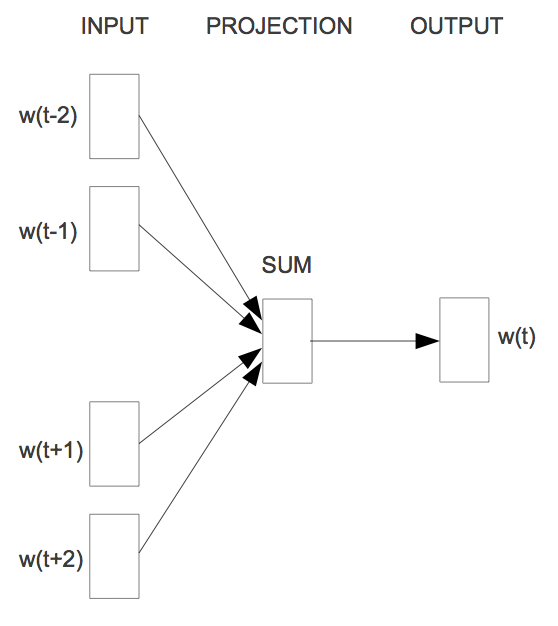
\includegraphics[width=0.5\textwidth]{./graph/cbow.png}\\
  \caption{词袋模型\cite{word2vec}}\label{fig:cbow}
\end{figure} 

模型的思路非常简单,用当前单词$w_t$前后窗口的词语去预估当前词$p(w_t \: | \: w_{t-n} , \cdots w_{t+n})$,那么整个语料的概率就是:
\begin{equation}
p(w_1 , \cdots , w_T) = \prod\limits_i p(w_i \: | \: w_{i-n} , \cdots , w_{i+n})
\end{equation}

同时可以计算整个模型的似然度为:
\begin{equation}
J_\theta = \frac{1}{T}\sum\limits_{t=1}^T\ \text{log} \space p(w_t \: | \: w_{t-n} , \cdots , w_{t-1}, w_{t+1}, \cdots , w_{t+n})
\end{equation}

如果基于n-gram的思想,这个时候,计算一个单词的概率就是基于这个单词组成的n-grams的频率,即:
\begin{equation}
p(w_t \: | \: w_{t-n} , \cdots , w_{t+n}) = \dfrac{count(w_{t-n}, \cdots , w_{t+n})}{count({w_{t-n}, \cdots , w_{t-1}, w_{t+1},\cdots, w_{t+n}})}
\end{equation}

我们可以通过softmax层来计算数学等价的一个概率:
\begin{equation}
p(w_t \: | \: w_{t-n} , \cdots , w_{t+n}) = \dfrac{\text{exp}({h^\top v'_{w_t}})}{\sum_{w_i \in V} \text{exp}({h^\top v'_{w_i}})}
\end{equation}

这里$V$和$h$都是我们需要学习的参数,每个单词$w$对应有两组参数,一组$v_w$是我们最终需要得到的词嵌入表示,另一组$h_w$是我们需要学习的隐层向量。
CBOW和Bengio提出的语言模型相比,唯一的改变就是Bengio的模型通过$w_t$之前的n个词来预测$w_t$而CBOW在每一个词$w_t$用其前后窗口$n$的词来做预测。
\subsubsection{skip-gram模型结构}
虽然CBOW可以被看作是一种预认识语言模型,但是skip-gram却改变了语言模型的目标:skip-gram使用中心词来预测周围的词,而不是像CBOW一样使用周围词预测中心词。
   \begin{figure}[h]
\centering
  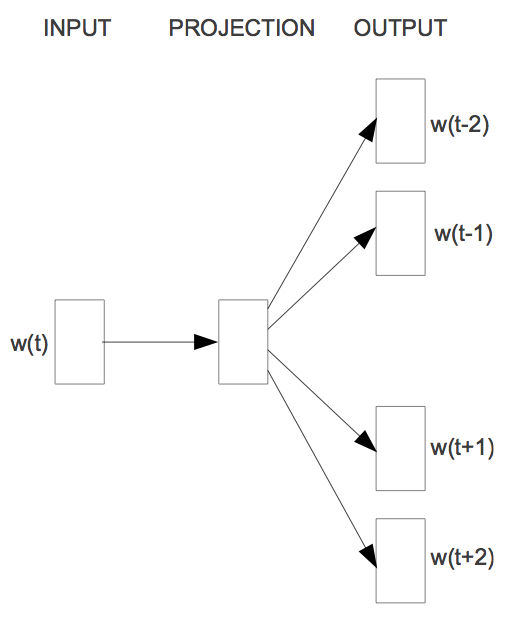
\includegraphics[width=0.5\textwidth]{./graph/skip-gram.png}\\
  \caption{skip-gram模型\cite{word2vec}}\label{fig:skip}
\end{figure} 
如图\ref{fig:skip}所示,skip-gram的似然度是非常简单的将$w_t$前后的$n$个词的似然度相加:
\begin{equation}
J_\theta = \frac{1}{T}\sum\limits_{t=1}^T\ \sum\limits_{-n \leq j \leq n , \neq 0} \text{log} \space p(w_{t+j} \: | \: w_t)
\end{equation}
同样的softmax被定义为:

\begin{equation}
p(w_t \: | \: w_{t-1} , \cdots , w_{t-n+1}) = \dfrac{\text{exp}({h^\top v'_{w_t}})}{\sum_{w_i \in V} \text{exp}({h^\top v'_{w_i}})} 	
\end{equation}

不再去计算给出其先前词语后目标词$w_t$的概率,我们计算给定$w_t$的周围词语$w_{t + j}$的概率。因此,我们可以简单地在方程中替换这些变量:
\begin{equation}
(p(w_{t+j} \: | \: w_t ) = \dfrac{\text{exp}({h^\top v'_{w_{t+j}}})}{\sum_{w_i \in V} \text{exp}({h^\top v'_{w_i}})}	
\end{equation}

同时skip-gram也不再如CBOW一样需要一个隐层的状态向量$h$,在这里$h$就是我们目标单词$w_t$的输入嵌入表示$v_{w^t}$,而我们最终得到的用于使用的目标单词$w_t$的输出向量定义为$v'_{w^t}$,将变量替换后:

\begin{equation}
p(w_{t+j} \: | \: w_t ) = \dfrac{\text{exp}({v^\top_{w_t} v'_{w_{t+j}}})}{\sum_{w_i \in V} \text{exp}({v^\top_{w_t} v'_{w_i}})}	
\end{equation}
\section{本章小结}
此章节主要介绍了推荐系统和词嵌入算法的发展,介绍了现有的推荐系统的一些已有算法和简单介绍存在的一些问题。之后介绍了词嵌入的思想和发展过程并具体介绍了词嵌入中比较流行的word2vec算法。为后文讨论主题模型和词嵌入与推荐系统的创新结合做好铺垫。
\chapter{主题模型和词嵌入(word embedding)与推荐系统的创新结合}
本章会首先会讨论主题模型和词嵌入算法可以为推荐系统带来提高的空间,以及具体能解决哪些方面的问题,并在之后会详细的介绍其应用场景和应用方法。
\section{主题模型和词嵌入(word embedding)在推荐系统中应用讨论}
推荐系统发展到现在,已经开始在各个行业扮演着非常重要的角色,其地位不言自明。这个领域的技术可以说比较成熟了,因为从底层的数据流梳理到中层的算法应用以及最上层的实时工作引擎,都有了一套比较清晰的工作模式。但是也可以说不成熟,因为永远没有一个完美的系统,推荐系统总会有着各种各样需要解决的问题,如冷启动问题\cite{Schafer2007}、同义的语义漂移问题\cite{synonymy}、作弊攻击问题\cite{shillingattacks}、长尾数据问题\cite{Longtail}以及数据和计算规模问题。

本文中我们主要聚焦于主题模型和词嵌入算法在推荐系统中的应用,因此在这里我们主要讨论其可应用的场景以及能解决的问题,主题模型和词嵌入算法的最终目标可以看做是提炼出对于单词和文档的连续向量表示,那么这个表示能再推荐系统中解决的问题是冷启动、长尾数据问题、以及稀疏计算存储规模问题。

\subsection{多场景的冷启动问题}
在各个行业的推荐系统,其应用场景都是多样的,如商品推荐系统,在淘宝这样的大生态体系下,其需要推荐的场景非常之多。比如营销活动时的推荐,日常的猜你喜欢,购物链路上的推荐。这些场景是不同的,传统的推荐系统依赖的点击率预估技术,或者是协同过滤技术会有一个问题,他们依赖的样本量巨大。而一个新的场景开始运转时,其积累样本是需要时间的。但是如果我们随机的为用户推送商品,这样积累数据的效率也非常低,因为用户往往看见的是自己不感兴趣的商品,这样场景的用户流失率会增大以后用户就不再登陆这个场景了。因此多场景的冷启动尤为关键,如何在初始时就尽快的积累有效的样本。

这时候主题模型和词嵌入算法的优势就得以体现出来。无论是主题模型还是词嵌入算法,其目标是根据已有数据得到对单词和文档有效的连续向量表达,这个向量是面向于潜层语义的。在商品推荐领域,我们可以将每一个商品(item)看做是一个单词(word),一个用户(User)的行为链(即其有过行为的item列表)看做是文档(doc),这样就能简单的使用主题模型和词嵌入算法来对商品和用户进行向量表达。而主题模型和词嵌入算法都有一个特性,就是其抽取的向量表达的可迁移性即强泛化性。我们从一个已有的良好运转的场景中去收集用户(user)以及商品(item)的数据,从这些已有的数据中去通过主题模型和词嵌入算法推断商品和用户的向量表达,这些向量表达在新的场景中也是有一定效果的。对比传统的点击率预估技术,其工业界应用做法大量的是使用稀疏的ID化逻辑回归模型,这样的模型的好处是其对高频样本的强拟合性,但是回到当前问题上,其模型一旦在一个固有的场景训练好,到了另一个场景由于数据分布的迁移,整个模型会几乎完全失效。因此主题模型和词嵌入算法合理的应用能有效的改善多场景的冷启动问题。

\subsection{长尾数据问题}
这个问题和上一小节中提到的冷启动问题有一点共通之处,就是其问题的本质是样本不够充足。不同之处在于,长尾数据问题中是有一部分的样本非常充足,而低频样本的贫乏导致了这些样本所代表的真实情形往往在推荐系统中被估计错误或偏移,而推荐系统又是一个非常强的自反馈系统有强马太效应,导致了推荐系统对那些低频数据处理得越来越差,一直无法让长尾数据得到有效的解决。更有意思的是,在商品推荐领域中长尾数据的占比还非常大,其分布也更为复杂,如图\ref{fig:LongTail}。
\begin{figure}[!h]
\centering
  \includegraphics[width=1.0\textwidth]{./graph/LongTail.png}\\
  \caption{商品推荐中的长尾效应}
\label{fig:LongTail}
\end{figure}

长尾分布式常见的,分布本身不会造成问题,造成问题的是常见的推荐系模式。如图\ref{fig:Sample},常见的推荐系统的样本分布空间分为三部分,训练样本空间、在线需要推断的样本空间以及全量样本空间。如果我们将一个用户(user)和一个商品(item)组成的对称为一个样本,训练样本空间即我们可以观测到的有反馈行为(点击与否,购买与否,收藏与否等等)的样本对,这个量是由推荐系统所服务的场景的用户使用情况有关的,同时全量样本空间是非常大的其数量等于用户数乘以商品数,远远大于训练样本空间,因为不可能所有的用户都对所有的商品做出过反馈。而在线需要推断的样本空间指的是在线系统中一个用户发送了请求之后,推荐系统需要给出的推荐分数,或者排序关系的样本对即给每个用户最终结果之前的商品候选集和用户间组成的样本。值得注意的是,这个数量也一定比训练样本空间大,因为推荐系统往往是在全量样本空间中通过一些match的方法,缩小了候选集之后,再用更精细的模型去进行筛选。而最终通过筛选出的商品被用户看到,并作出反馈行为,成为系统可以收集的训练样本,未被用户看到的样本推荐系统其实无法定义这些样本的性质(label)。

清晰了推荐系统的样本分布之后,其实长尾问题带来的影响就明确了,那些活跃的商品,会被系统推送出展现更多的次数,与此同时这些活跃的商品就更多的进入了训练样本空间,推荐系统对这些商品的学习变得更精准。反之那些低频的商品就更少的被展现,推荐系统也就更难收集到这些商品的样本进行学习,对这些商品的评价就越来越不精准。这样的一个反馈系统,会让用户总是看到一些热门的商品,这会极大的损伤用户的体验。

而如上一小节提到,主体模型和词嵌入学习算法通过合理的设计能具有较强的泛华性。并且这两种算法思路在定义模型的时候,不会以商品和用户组成的对为单位来定义样本,其样本是行为列表,这个不同会使得这些方法更好的学习到每个商品和每个用户的潜层语义,因此值得尝试用主题模型和词嵌入学习的思路来解决长尾问题。
\begin{figure}[!h]
\centering
  \includegraphics[width=1.0\textwidth]{./graph/Sample.png}\\
  \caption{推荐系统的样本分布}
\label{fig:Sample}
\end{figure}

\subsection{稀疏数据的计算存储规模问题}
推荐系统抽象出来的问题是对一个用户推荐一些商品,或者将一个商品推荐给可能感兴趣的用户群体,而系统中用于表达用户的特征是用户对各种商品的行为,对商品的表达是在这个商品上有过各种行为的用户列表。这样的数据是由次数和代表用户或者商品的ID组成的,是非常宽维度并且稀疏的,实际应用中往往使用哈希的方法来存储,但是其开销的空间是巨大的。而且真实的在线系统中虽然哈希的方法在取一个ID对应值的复杂度可以认为是$O(1)$,但是这个开销也和用户的行为次数呈线性相关。

如果现在每个用户和每个商品都用一个固定维度的连续向量表达,这样对系统无论从计算还是存储方面带来的便利性都是极大的。
\section{主题模型在推荐系统中的结合}
如前文中提到,将每个用户(user)的行为列表(item list)看做是文档(doc),每个商品(item)定义为单词(word)就可以很简单的用主题模型对之建模。这节会详细的介绍在商品推荐问题上,如何对用户和商品进行建模,并得到它们的潜层概率空间语义表达。

主题建模的方法有很多,包括之前介绍的PLSA、LDA、非对称LDA以及我们在这篇论文中创新提出的HLSM。但是在真实的商品推荐场景下,对应于文档(doc)的用户量是亿级别的,对应于单词(word)的商品量也是亿级别的。这样的数据级别上,并行计算的PLSA是比较好的选择,而本文提出的HLSM由于其中需要对单词和文档共现矩阵进行非负矩阵分解,目前没有很好的资源能解决这一问题,同时LDA虽然有其并行计算版本PLDA\cite{PLDA}和MSRA提出的Light LDA\cite{lightLDA},但受资源限制选择设计了以PLSA为基础的方法。

和PLSA一样,这里我们要估计的是两个概率分布$p(topic|user)$(后文中简写为$p(t|u)$)与$p(item|topic)$(后文简写为$p(i|t)$)。则整个训练数据集的概率$p(item, user)$为:
\begin{equation}
P(\mathbf{item, user}) = \prod_{s=1}^N \prod_{j=1}^M P(u_s, i_j)^{n(u_s, i_j)}
\end{equation}
则似然度函数为:
\begin{equation}
\begin{split} \log P(\mathbf{u,i}) &= \sum_{s=1}^N \sum_{j=1}^M n(u_s, i_j) \log P(u_s, w_j) \\ &= \sum_{s=1}^N n(u_s) [\log P(u_s) + \sum_{j=1}^M \frac{n(u_s, i_j)}{n(u_s)} \log \sum_{k=1}^K P(i_j|t_k) P(t_k|u_s)] \\ & \propto \sum_{s=1}^N \sum_{j=1}^M n(u_s, i_j) \log \sum_{k=1}^K P(i_j|t_k) P(t_k|u_s) \\ \end{split} 
\end{equation}
用EM算法来进行推断,则对应的Q方法函数为:
\begin{equation} \begin{split} Q(\bm\theta|\bm\theta^{(i)}) &= \sum_{t_1, ..., t_n} \sum_{l=1}^n \log P(\mathbf{u,i},t_l) P(t_1, ..., t_n|\mathbf{u,i}) \\ &= \sum_{t_1,t_2,...,t_n} [ \log P(\mathbf{u,i},t_1) + ... + \log P(\mathbf{u,i},t_n)] \\ & \ \ \ \ \ \ \ \ \ \ \ \ \ \ \ P(t_1|\textbf{u,i}) P(t_2|\textbf{u,i}) ... P(t_n|\textbf{u}) \\ &= \sum_{t_1,t_2,...,t_n} [\log P(u_1,i_1,t_1) + ... + \log P(u_n,i_n,t_n)] \\ & \ \ \ \ \ \ \ \ \ \ \ \ \ \ \ P(t_1|u_1,i_1) P(t_2|u_1,i_1) ... P(t_n|u_1,i_1) \\ &= \sum_{s=1}^N \sum_{j=1}^M n(u_s, i_j) \sum_{k=1}^K P (t_k|u_s, i_j)\log P(i_j|t_k) P(t_k|u_s) \\ \end{split} \end{equation}
由此E step为:
\begin{equation}
P (t_k|u_s, i_j) = \frac{P(i_j|t_k)P(t_k|u_s)}{\sum_{l=1}^K P(i_j|t_l) P(t_l|u_s)}
\end{equation}
M step为:
\begin{equation}
P(i_j|t_k) = \frac{\sum_{s=1}^N n(u_s,i_j) P(t_k|u_s,i_j)}{\sum_{m=1}^M\sum_{s=1}^N n(u_s,i_m) P(t_k|u_s,i_m)}
\end{equation}
\begin{equation}
P(t_k|u_s) = \frac{\sum_{j=1}^M n(u_s,i_j)P(t_k|u_s,i_j)}{n(u_s)}
\end{equation}
其中$n(u_s)$表达的是用户i的行为次数。

而在真实的使用场景中,用户的行为列表会发生非常快的变化,如一个淘宝用户会不听的进行商品点击、购买、收藏等行为,其行为列表的更新频率非常的高。如果我们用上述公式中的$p(t|u)$来表示用户,这个概率分布是过去用户的潜层语义空间的表示,而不是当下用户实时的语义表示。而更为稳定的表达是对于商品的,因为商品本身的属性随时间迁移的变化并不会特别明显,至少在天级别的更替中,我们认为商品的属性不会发生太大的变化。所以在真实的使用过程中,我们仅仅固定了一个概率分布$p(t|i) = \frac{p(t) \cdot p(i|t)}{p(i)}$为商品的向量表达$Item_{vec}$,其中$p(t) = \frac{\sum_{s=1}^N p(t|u_s)}{N}$。将用户的向量表达$User_{vec}$定义为其所有行为列表中商品对应的$p(i|t)$的加权平均:
\begin{equation}
User_{vec} = \frac{\sum_{j=1}^M n(u,i_j)\overrightarrow {p(i|t)}}{n(u)}
\end{equation}
在获取到$User_{vec}$和$Item_{vec}$之后,我们可以定义一个函数$f(User_{vec}, Item_{vec})$来计算User和Item的相关性分数:
\begin{equation}
Score_{ui} = f(User_{vec}^u, Item_{vec}^i)
\end{equation}

最直观的,我们可以将之定义为余弦距离:
\begin{equation}
Score_{ui} = \cos User_{vec}^u \cdot Item_{vec}^i
\end{equation}

当然,我们做了更复杂一点的尝试,用一个深度神经网络来学习$f$,如图\ref{fig:Dnn}。这里可以用已经观测过有反馈的User和Item组成的pair样本来训练,如有点击label是1没有点击label为0。这么做的动机是因为$User_{vec}$和$Item_{vec}$的关系函数并不是已知的,而深度神经网络的拟合能力非常强,在有足够样本的情况下,其可以很好的拟合出$User_{vec}$和$Item_{vec}$的函数关系。不过缺点是其计算与训练的开销都不如之前提到的计算余弦距离那么直接。在之后的实验章节中会详细介绍这两种方法间的对比效果。
\begin{figure}[!h]
\centering
  \includegraphics[width=0.8\textwidth]{./graph/Dnn.png}\\
  \caption{User和Item关系学习的全连接神经网络}
\label{fig:Dnn}
\end{figure}

综上所述,主题模型在推荐系统中应用的整个步骤为:
\begin{enumerate}[步骤 1.]
\item 将用户(User)的行为数据整理为商品链(Item list)作为文档,每个商品作为单词
\item 在上一步产出的数据中用PLSA通过EM算法去迭代推断$p(i,t)$
\item 计算$p(t) = \frac{\sum_{s=1}^N p(t|u_s)}{N}$ 和 $p(t|i) = \frac{p(t) \cdot p(i|t)}{p(i)}$
\item 存储$\overrightarrow p(t|i)$ 为 $Item_{vec}$
\item 计算$User_{vec} = \frac{\sum_{j=1}^M n(u,i_j)\overrightarrow {p(i|t)}}{n(u)}$
\item 在线对于$Item_i$和$User_u$通过定义好的函数$f(User_{vec}, Item_{vec})$计算$Score_{ui} = \cos User_{vec}^u \cdot Item_{vec}^i$
	
\end{enumerate}
本文在之后的实验章节中也会详细介绍在实际应用场景中对此种方法的尝试的环境以及最终的实验结果,由此来验证这一想法的有效性。
\section{类word2vec词嵌入方法在推荐系统中的结合}
这一小节将主要介绍类似word2vec这种和最终使用场景不直接相关的词嵌入方法在推荐系统中的结合,在下一小节将介绍本文提出的一种在推荐系统中和使用场景相关性稍强的弱监督词嵌入方法。

\subsection{基于用户行为序列的word2vec}
和前文分析一样,将用户在商品上的行为序列抽象为文档,则单词就是每一件商品。这里直观的去思考用户行为序列的生成过程,为了更好的去理解,本文摘取了一个实际的用户行为序列(已经人工的去掉了所有图例中的商标)用于展示。

如图\ref{fig:zuji1},可以发现用户的行为是有明显的局部连续一致性的,如果考虑到周围的商品之间的关系,可以看到在一定区域内商品相邻的商品是相似的。这个可以很直观的理解,一个用户在商城浏览的时候一定会在某一兴趣点上连续的浏览,直到选中自己心仪的商品或者被其他兴趣点相关的商品吸引开。此图中的最左端商品就可以看到,用户的兴趣从女鞋到了女裤。这里女鞋和女裤可以是搭配关系,也算有一定的相似性,如果简单的用n-gram信息进行学习也是能有收益的。可能拟合出具有这种搭配关系的兴趣迁移。

但是如图\ref{fig:zuji2},用户的兴趣可能是跳跃的,男裤之后是零食之后又到女鞋,这一行为的捕捉是非常困难的,这样的行为序列占比还非常大,而相邻的商品彼此之间可能出现兴趣的断点,如果在这里直接用n-gram去监督我们的word2vec显然是不合理的,因为在零食后面出现任何兴趣点都有可能,而这完全是噪声。

为了避免这些噪声,需要先研究清楚这种噪声的分布情况。根据消费者进入网络商城的目标是要选择或者只是观察自己想要的商品,而兴趣的巨大跳跃是和时间有关系的,人在短时间之内去大尺度的改变一个兴趣点的可能会比较小。但是直观的理解显然是不严谨的,因此本文为了探索时间和兴趣点迁移的关系做了严谨的数据统计。

统计的目标很简单,本文在这里认为跨类目粗略算作是兴趣点的迁移,统计两次行为之间相邻时间长短$\Delta T$和两次行为商品属于不同类目的比例$\delta$,对用户的行为做抽样统计了两者间的关系,如图\ref{fig:TimeDelta}。

从图中我们可以看到两次行为的商品跨类目比例$\delta$与两次行为的时间间隔$\Delta T$成递增关系并且是一个类对数分布。这说明之前的直观理解和实际的数据分布是相符合的。
\begin{figure}[!htp]
\centering
  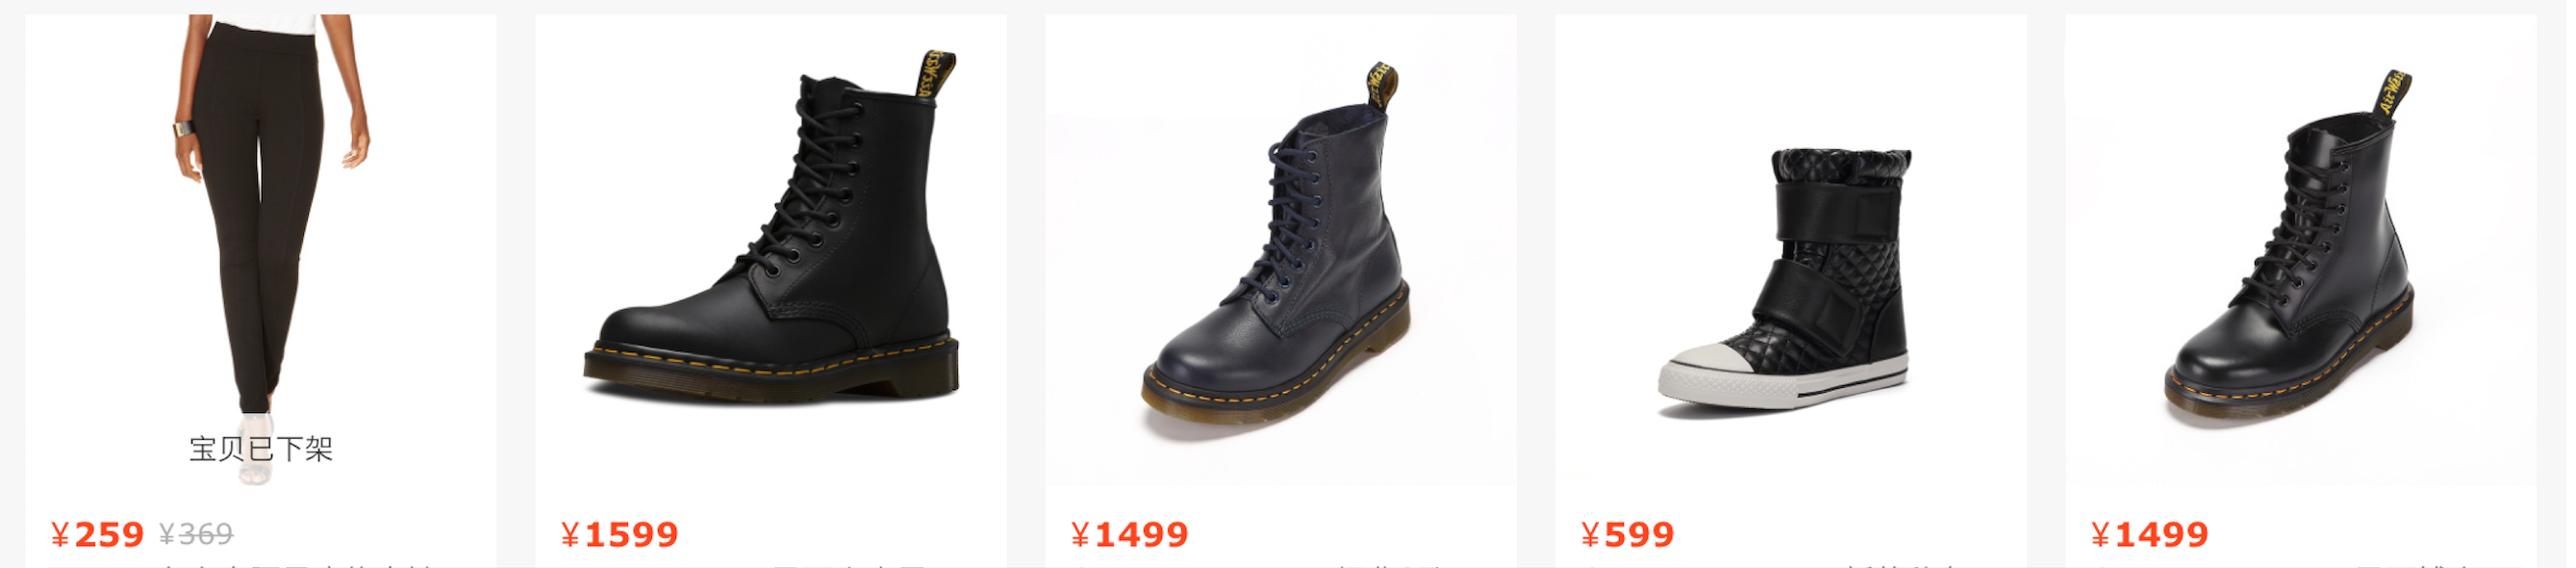
\includegraphics[width=0.8\textwidth]{./graph/zuji1.png}\\
  \caption{网络商城中用户的行为足迹1}
\label{fig:zuji1}
\end{figure}
\begin{figure}[!htp]
\centering
  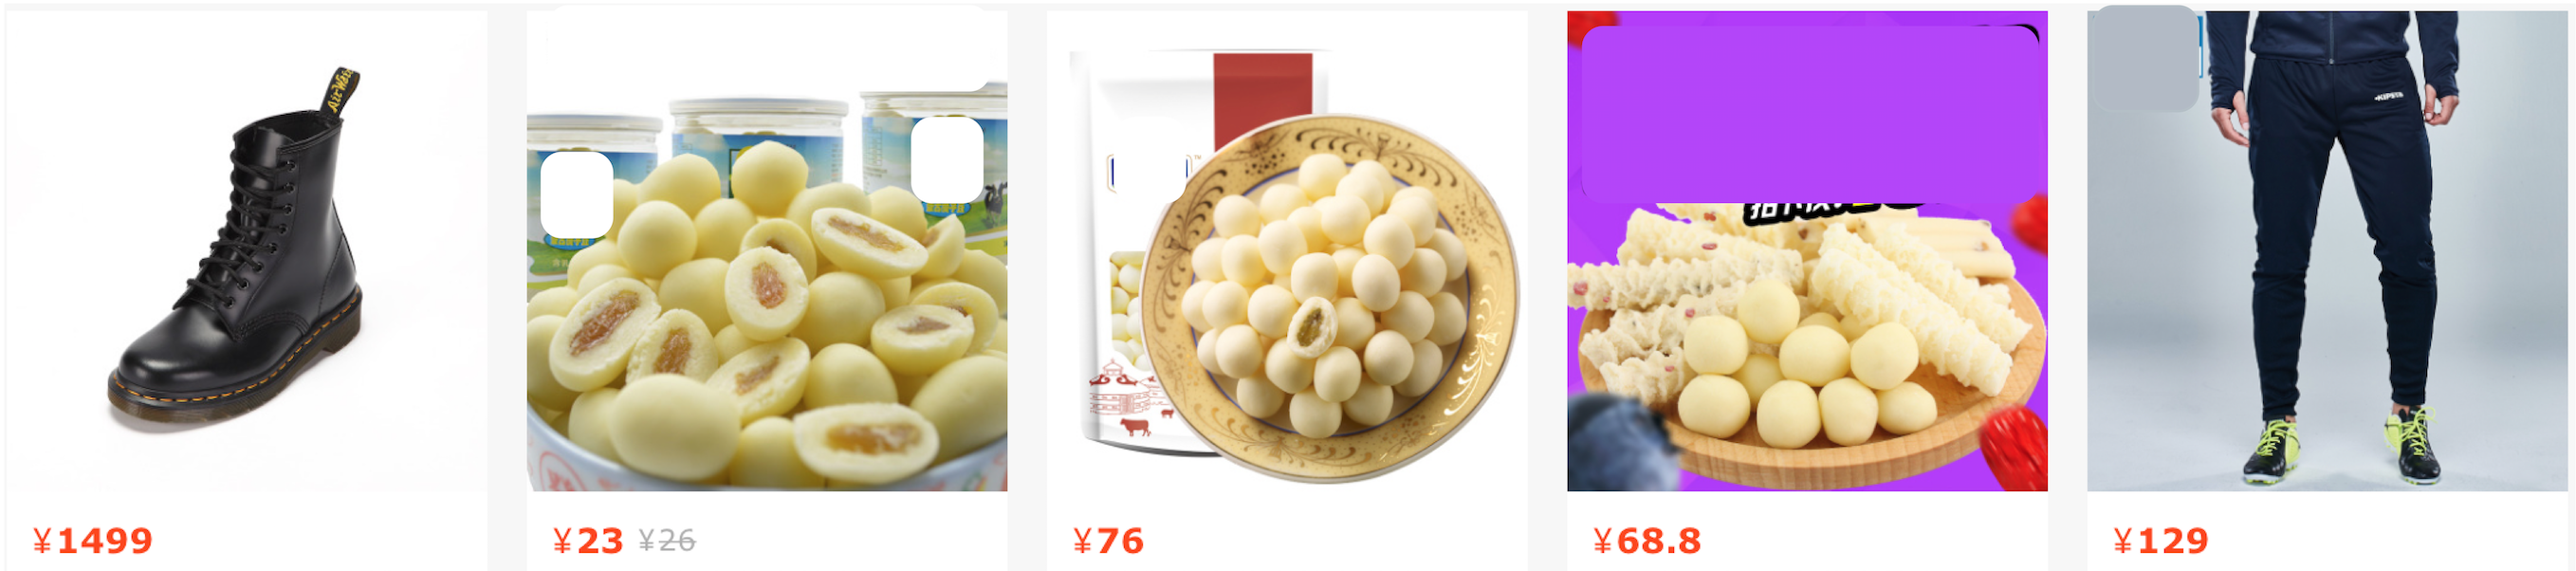
\includegraphics[width=0.8\textwidth]{./graph/zuji2.png}\\
  \caption{网络商城中用户的行为足迹2}
\label{fig:zuji2}
\end{figure}
\begin{figure}[!htp]
\centering
  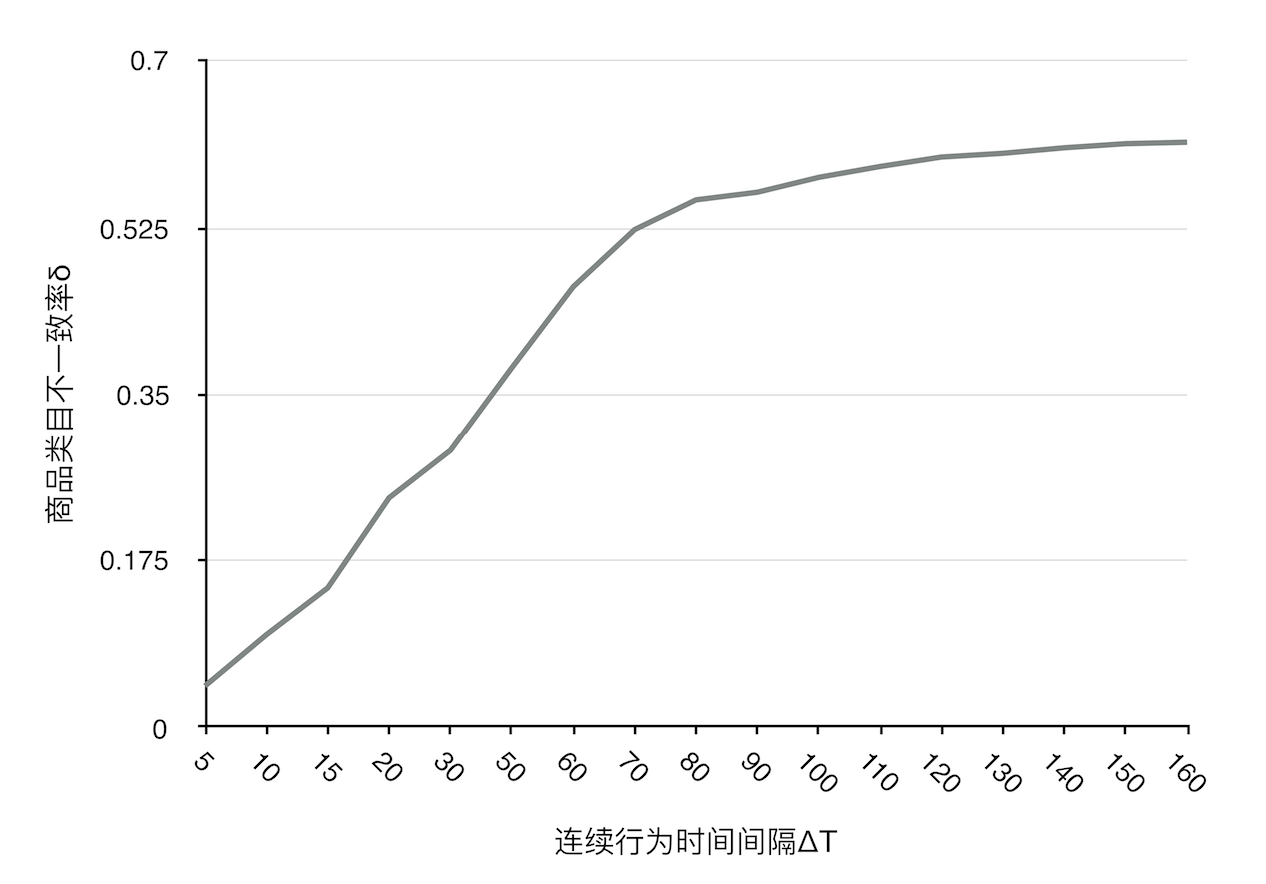
\includegraphics[width=0.8\textwidth]{./graph/TimeDelta.png}\\
  \caption{两次连续行为跨类目比例和时间间隔的关系分布}
\label{fig:TimeDelta}
\end{figure}
%% 本章参考文献
\ifx\usechapbib\empty
\nocite{BSTcontrol}
\setcounter{NAT@ctr}{0}
\bibliographystyle{buptgraduatethesis}
\bibliography{bare_thesis}
\fi
